\usetikzlibrary{calc}
\subsection{The Morris Worm}

\begin{frame}[plain]
    \begin{tikzpicture}[remember picture,overlay]
        \node[at=(current page.center)] {
            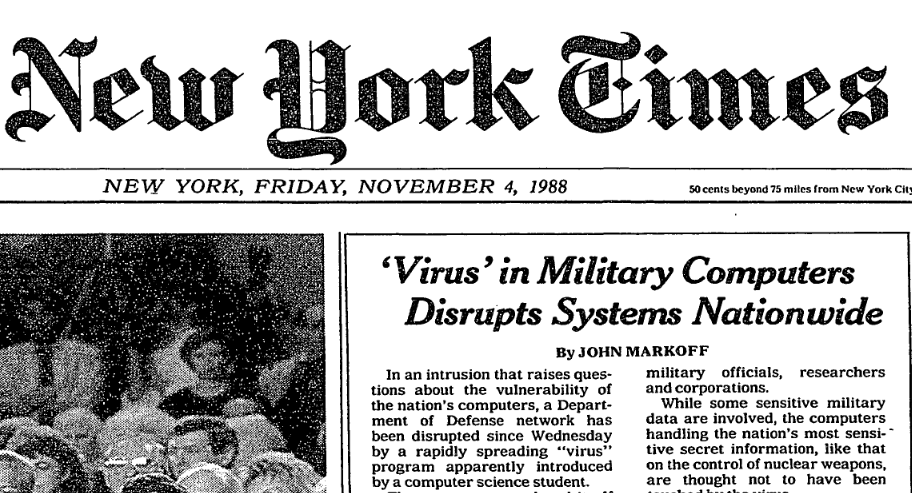
\includegraphics[width=\paperwidth]{../intro/nyt-head-virus}
        };
    \end{tikzpicture}
\end{frame}

\begin{frame}[plain]
    \begin{tikzpicture}[remember picture,overlay]
        \node[at=(current page.center)] {
            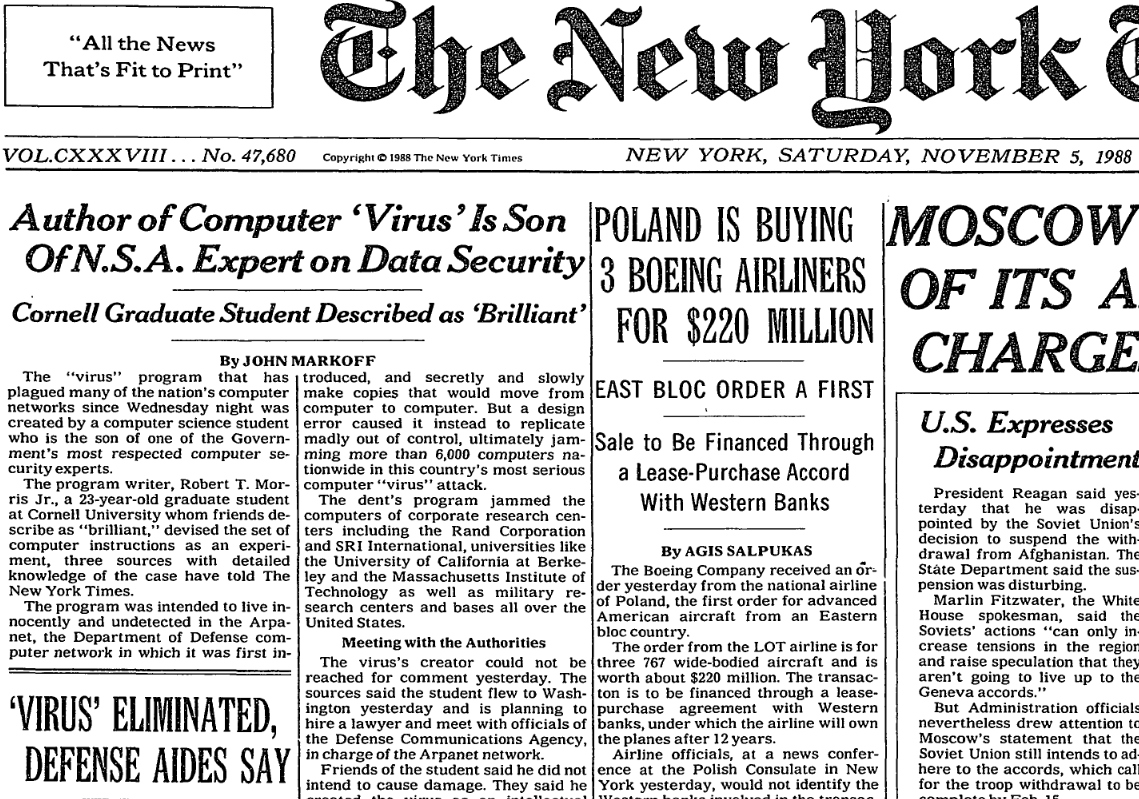
\includegraphics[width=\paperwidth]{../intro/nyt-head-morris}
        };
    \end{tikzpicture}
\end{frame}

\begin{frame}{Morris worm mechanisms}
\begin{itemize}
    \item used vulnerabilities in some versions of:
        \begin{itemize}
        \item mail servers ({\tt sendmail})
        \item user information servers ({\tt fingerd})
        \end{itemize}
    \item also spread using {\tt rsh}/{\tt rexec} (predecessor to ssh)
    \item hid by being called {\tt sh} (default shell)
    \item strings obscured slightly in binary
\end{itemize}
\imagecredit{Eichin and Rochlis, ``With Microscope and Tweezers: An Analysis of the Internet Virus of November 1998''}
\end{frame}

\begin{frame}{the early Internet}
    \begin{itemize}
    \item pretty homogeneous --- almost all Unix-like systems
    \item {\tt sendmail} was ``the'' email server to run
    \item most institutions vulnerable
    \end{itemize}
\end{frame}

\begin{frame}{Morris worm intent versus effect}
\begin{itemize}
\item code in viruses tried to avoid ``reinfecting'' machines
\item \ldots{} but not actually effective
\end{itemize}
\end{frame}


